\documentclass[12pt,a4paper]{article}
\usepackage[marginparsep=8pt,left=2.5cm,right=2.5cm,top=2.5cm,bottom=3cm]{geometry}
\usepackage{graphicx}% http://ctan.org/pkg/graphicx
\usepackage{titlesec}
\usepackage{xcolor}

\usepackage[utf8]{inputenc}
\usepackage[T1]{fontenc}
\usepackage{fontspec}

\setmainfont[ExternalLocation=Fonts/]{Calluna-Regular.otf}[
  BoldFont=Calluna-Bold.otf,
  ItalicFont=Calluna-It.otf,
  BoldItalicFont=Calluna-BoldIt.otf
]

\setlength{\parindent}{0pt}% Remove paragraph indent



\begin{document}
\pagenumbering{gobble}

\titleformat{\subsection}
   {\color{black}\normalfont\fontsize{13}{18}\bfseries}{\thesection}{1em}{}

%\titlespacing*{\subsection}{0cm}{0.6cm}{-0.2cm}


\center{\textbf{\fontsize{25}{30}\selectfont R-tree}}
\center{{\fontsize{14}{30}\selectfont Pavel Jahoda}}
\center{{\fontsize{12}{30}\selectfont \today}}\\[1.5cm]
%\title{\Huge R-tree}
%\author{\large Pavel Jahoda}
%\date{\normalsize \today}
%\maketitle

\flushleft\subsection*{Popis Projektu}
%\setlength{\parindent}{20pt}% Remove paragraph indent
Cílem projektu je vytvoření vlastní perzistentní implementace R-stromu, což je stromová struktura pro vyhledávání n-dimenzionálních objektů často využívaná v geografických informačních systémech. Řešení překonává požadavky zadání a kromě dotazů nad databází 2D nebo 3D objektů, zvládá i požadavky na n-dimenzionální objekty. Dotazovat se lze jak na nejbližšího souseda, tak na rozsahových dotazem (tj. které objekty jsou K jednotek daleko od bodu X). Aplikace obsahuje testovací modul, který si dokáže generovat náhodná data tak i pracovat s ručně zadanými daty. Testovací modul kontroluje vyváženost stromu, korektnost velikosti bounding boxů, také testuje dotazování na nejbližšího sousedu a rozsahové dotazy \\[0.6cm]
Navíc oproti zadání, které umožnuje generování náhodných dat (které generuji v testovacím modulu), stahuji data z aplikace flightradar od která s 5 minutovým spožděním získávám data o letištích a také letadlech, která jsou v daný moment ve vzduchu. Kromě polohy získávám rychlost, typ letadla, leteckou společnost ke které letadlo patří a další zajímavé údaje. Kromě náhodných dat je tedy možné se dotazovat i na letecká data.  \par \bigskip

\subsection*{Způsob řešení}
Lorem ipsum dolor sit amet, consectetur adipiscing elit, sed do eiusmod tempor incididunt ut labore et dolore magna aliqua. Ut enim ad minim veniam, quis nostrud exercitation ullamco laboris nisi ut aliquip ex ea commodo consequat. Duis aute irure dolor in reprehenderit in voluptate velit esse cillum dolore eu fugiat nulla pariatur. Excepteur sint occaecat cupidatat non proident, sunt in culpa qui officia deserunt mollit anim id est laborum\par \bigskip

\subsection*{Implementace}
Lorem ipsum dolor sit amet, consectetur adipiscing elit, sed do eiusmod tempor incididunt ut labore et dolore magna aliqua. Ut enim ad minim veniam, quis nostrud exercitation ullamco laboris nisi ut aliquip ex ea commodo consequat. Duis aute irure dolor in reprehenderit in voluptate velit esse cillum dolore eu fugiat nulla pariatur. Excepteur sint occaecat cupidatat non proident, sunt in culpa qui officia deserunt mollit anim id est laborum\par \bigskip

\subsection*{Příklad výstupu}

\subsection*{Experimentální Sekce}
R-strom nabízí hned několik věcí na testování. Z hlediska rychlost vkládání prvků a následných dotazů můžeme porovnávat vliv různých metod dělení ůzlů, počet potomků uzlu, počet dimenzí nebo vzdálenost u rozsahového dotazu.\\[0.5cm]
Tabulka níže (Table 1) ukazuje vliv volby metody dělení ůzlů (když uzel dosáhl maximálního množství potomků) na rychlost vkládání prvků a rychlost rozsahových dotazů. Data v tabulce jsou zprůměrováná z pěti různých testování na stromu s maximálním množstvím 8 potomků na uzel, na trojdimenzionálních datech na 2 000 datech a 20 000 dotazech. Data jsou v sekundách.
 
\begin{table}[ht]
\begin{center}
\caption{Rychlost vkládání a dotazů}
\label{tbl:bins} % spaces are big no-no withing labels
\begin{tabular}{|c|cc|} 
\hline
\multicolumn{1}{|c}{} & \multicolumn{1}{c}{Insert} & \multicolumn{1}{c|}{Query} \\
\hline
Random & 1.0669 &   19.45292 \\
\hline
Brute force & 4.73896 &   5.33882 \\
\hline
Heuristic & 0.91115 &   7.51662 \\
\hline
\end{tabular}
\end{center}
\end{table}

Výsledek je očekávaný. Metoda hrubou silou (brute force) je jasně nejpomalější pří vkládání, zatímco na dotazech vyhrává. Metoda dělení heuristikou nejenže nejrychleji vkládá prvky, ale vede si obstojně i v rozsahových dotazech, což je důvodem proč jsou heuristiky na R-stromech používané. Na druhou stranu metoda náhodného rozdělení uzlů je suveréně nejhorší na rozsahové dotazy.\\[0.5cm]
Na grafu níže můžeme pozorovat vliv počtu potomků uzlu na dobu vkládání prvků. Zatímco vkládání s dělením ůzlu heuristikou nebo náhodným dělením je s vzrůstajícím počtem potomků dokonce neptrně rychlejší tak u dělení hrubou silou můžeme pozorovat velký pokles rychlost přidávání. Tento fakt je způsoben tím, ze řešení hrubou silou skouší všechny možné permutace rozdělení uzlu, což je asymptoticky exponenciální.

\begin{center}
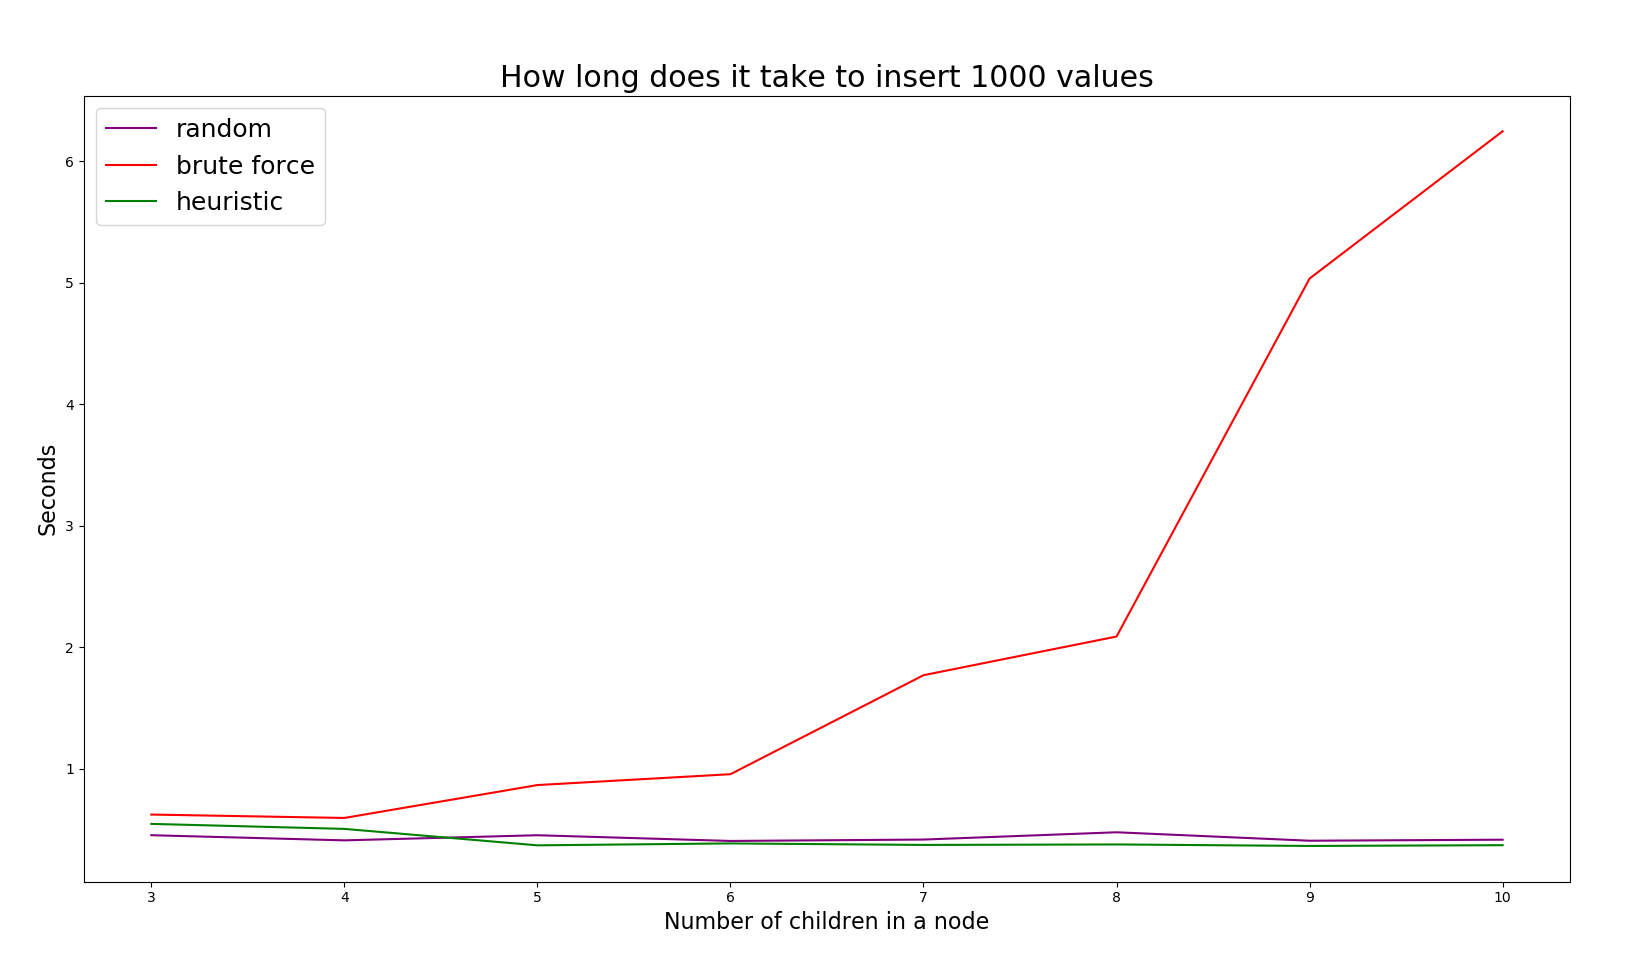
\includegraphics[width=15cm, height=8cm]{nOfChildren}
\end{center}

Na závěr experimentální sekce bych zde uvedl, že počet dimenzí hraje naprosto minimální vliv na rychlost vkládání nebo na rychlost rozsahových dotazů. Toto zjistění potvrzuji silné stránky R-stromu.

\subsection*{Diskuze}

\subsection*{Závěr}

\end{document}
